\documentclass[12pt]{article}

\usepackage{graphicx}
\usepackage{minted}
\usepackage[margin=3cm]{geometry}

\graphicspath{ {./} }

\author{Pablo Vargas Bermúdez}

\begin{document}
\pagestyle{empty}

\section*{Planteamiento}

Poner botones en una ventan los cuales no se tienen que dejar hacer
click, se tienen que mover cuando el usuario posicione su puntero
encima de cierto botón.

\section*{Código}

\subsection*{Clase Botones Locos}

\inputminted{Java}{CrazyButtons.java}

\subsection*{Clase de Prueba}

\inputminted{Java}{Prueba.java}

\section*{Ejecución}

\subsection*{Inicio}

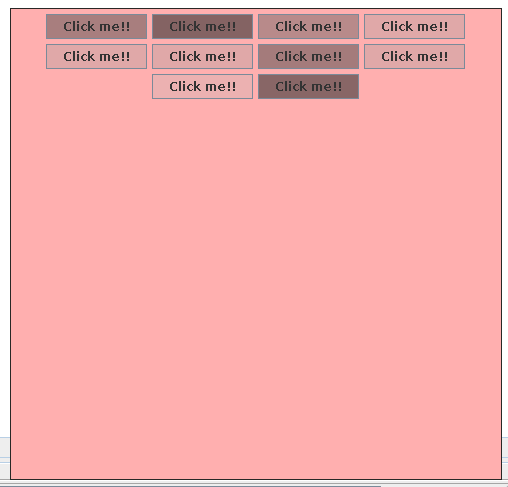
\includegraphics[width=\textwidth]{Ejecucion3.png}

\subsection*{Después de mover el ratón}

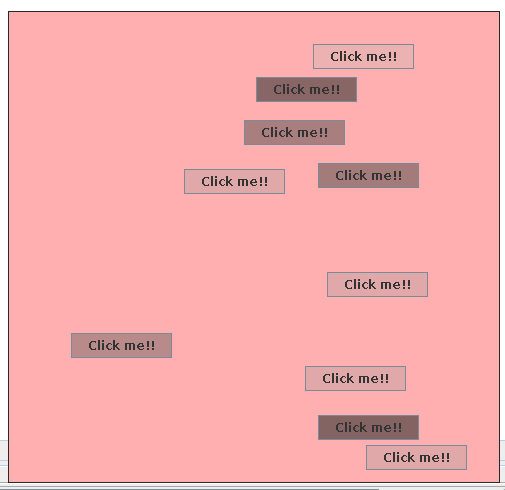
\includegraphics[width=\textwidth]{Ejecucion1.png}

\subsection*{después de mover más el ratón}

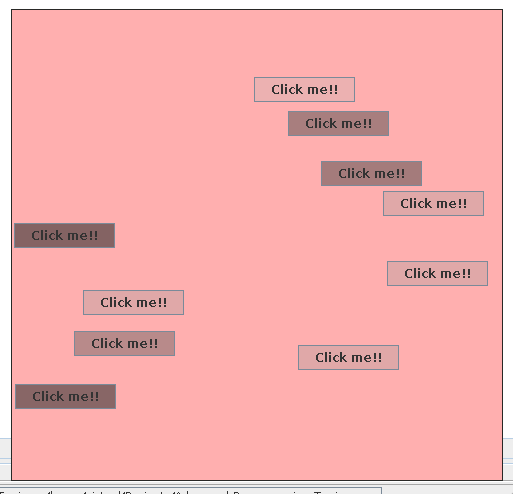
\includegraphics[width=\textwidth]{Ejecucion2.png}

\end{document}
